\subsection{基本内存分配实验}
\subsubsection{运行环境}
程序在以下环境下构建和测试.
\begin{description}
    \item[操作系统] macOS 13.1 22C5044e arm64;
    \item[c编译器] gcc (Homebrew GCC 12.2.0) 12.2.0;
    \item[构建和测试工具] GNU Make 3.81;
    \item[文档编译工具] XeTeX 3.141592653-2.6-0.999994 (TeX Live 2022)
    \item[文本编辑器] nvim v0.8.1
    \item[调试工具] Visual Studio Code Version: 1.74.0 (Universal),
        lldb-1400.0.38.13
\end{description}

\subsubsection{程序运行方式}
程序使用make进行构建和测试. 读者优先程序和写者优先程序都会被构建在build/目录下.\par
对于程序的构建, 执行如下命令.
\begin{code}
    make
\end{code}

对于程序的执行, 可以使用如下命令:
\begin{code}
    build/main
\end{code}

建议使用测试的方式运行模拟程序, 使用以下命令:
\begin{code}
    make test FROM=0 TO=1000 NUM_BLOCKS=1000 NUM_PROCESSES=100
\end{code}
在这种情况下, 将会先使用数据生成器data\_gen根据后面的参数生成配置文件到
config/config.txt, 然后再执行程序. 在参数中, FROM和TO指定进程请求内存大小和内存
孔大小的下界和上界, NUM\_BLOCKS指定内存孔的数量, NUM\_PROCESSES指定请求内存的进
程的数量.\par

之后程序会读取config/config.txt配置文件, 加载进程数量, 每个进程请求内存大小, 内存
孔数量, 每个内存孔大小. 进入后可以看到菜单如下, 输入对应标号可以进入对应界面.

\begin{lstlisting}[language=c++]
    MEMORY MANAGEMENT ALLOCATION SIMULATION
    Options:
    0. Customize configuration
    1. First Fit
    2. Best Fit
    q. Exit
\end{lstlisting}

\begin{itemize}
    \item 输入0可以重新设置进程数量, 每个进程请求内存大小等内容. 设置仅对本次执行有效.
    \item 输入1将模拟First Fit分配.
    \item 输入2将模拟Best Fit内存分配.
    \item 输入q将退出程序.
\end{itemize}

\subsubsection{程序日志格式}
程序将随内存分配将分配结果输出到console. 格式为
\begin{code}
    process[<pid>] in block[<bid>] <psize>/<bsize>
\end{code}
其中, pid为进程id, bid为内存孔id, psize为进程申请空间大小, bsize为内存孔大小.\par

如果进程没有合适的孔可以分配, 则输出日志
\begin{code}
    process[<pid>] is not assigned.
\end{code}

在内存分配结束后, 将输出内部碎片和外部碎片统计信息, 例如
\begin{code}
    ------FRAGMENTATION STATISTICS------

    Total internal fragmentation: 10910
    Total external fragmentation: 7283
\end{code}
表示总的内部碎片大小为10910字节, 外部碎片大小为7283字节.

\subsubsection{运行结果}

\begin{code}
    # Build
    make test FROM=0 TO=1000 NUM_BLOCKS=1000 NUM_PROCESSES=1000

    # Run First fit simulation.
    1

    # Run Best fit simulation.
    2

    # Exit.
    q
\end{code}

设定进程申请内存大小和内存孔大小范围在0到1000的情况下,
\begin{itemize}
    \item 10000进程, 10000个内存孔First fit的内部和外部碎片统计如图~\ref{fig:10000p10000b-first}.
    \item 10000进程, 10000个内存孔Best fit的内部和外部碎片统计如图~\ref{fig:10000p10000b-best}.
    \item 5000进程, 10000个内存孔First fit的内部和外部碎片统计如图~\ref{fig:5000p10000b-first}.
    \item 5000进程, 10000个内存孔Best fit的内部和外部碎片统计如图~\ref{fig:5000p10000b-best}.
    \item 10000进程, 5000个内存孔Best fit的内部和外部碎片统计如图~\ref{fig:10000p5000b-first}.
\end{itemize}

\begin{figure}[ht!]
    \centering
    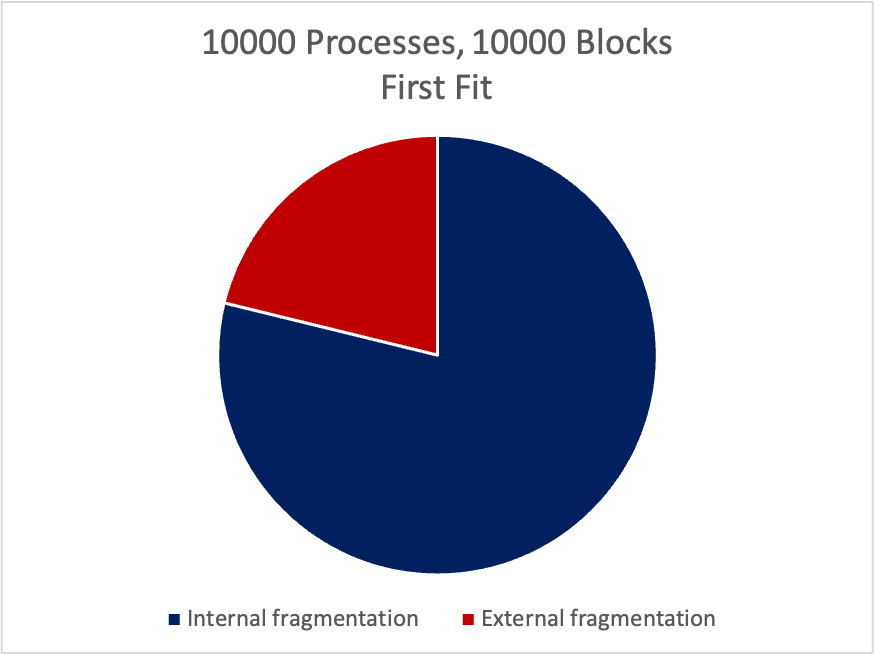
\includegraphics[width=0.95\textwidth]{10000b-10000p-first-fit.png}
    \caption{10000进程,10000内存孔First Fit}
    \label{fig:10000p10000b-first}
\end{figure}

\begin{figure}[ht!]
    \centering
    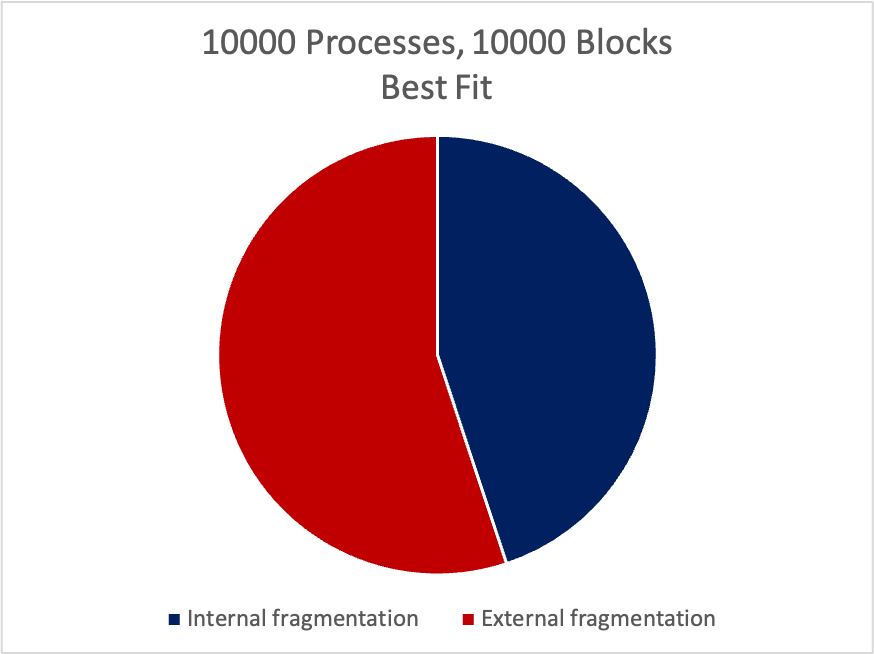
\includegraphics[width=0.95\textwidth]{10000b-10000p-best-fit.png}
    \caption{10000进程,10000内存孔Best Fit}
    \label{fig:10000p10000b-best}
\end{figure}

\begin{figure}[ht!]
    \centering
    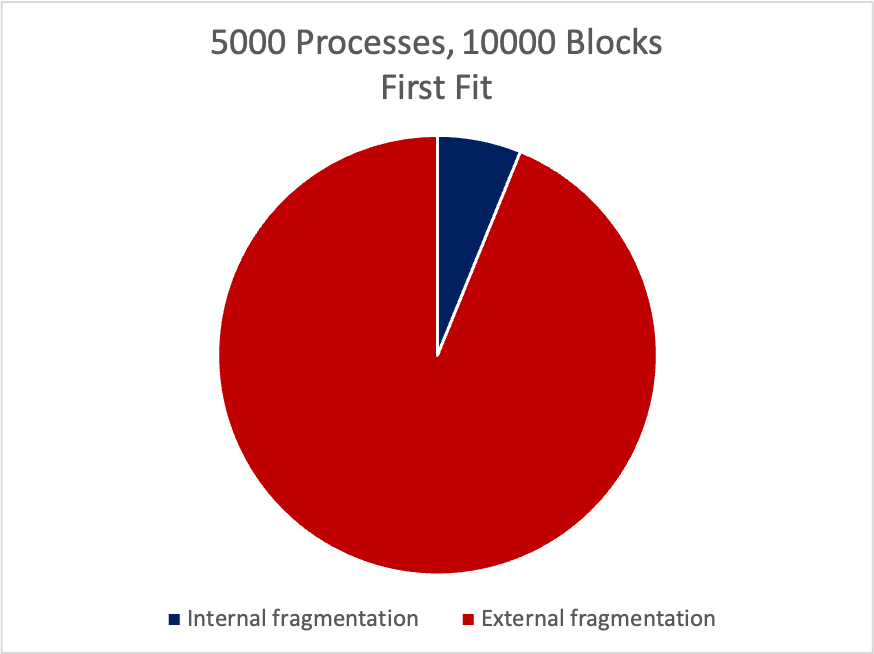
\includegraphics[width=0.95\textwidth]{10000b-5000p-first-fit.png}
    \caption{5000进程,10000内存孔First Fit}
    \label{fig:5000p10000b-first}
\end{figure}

对比进程数和内存孔数均为10000的情况下的First Fit和Best Fit, 可以发现在进程的总大
小和所有内存孔的总大小相同的情况下, First Fit的Internal Fragmentation相比Best
Fit方法的开销大得多.\par

而在进程数远少于内存孔的5000进程10000内存孔的情况下, Best Fit能几乎完全的消除内
部碎片, 而First Fit仍有不小数量的内部碎片存在.\par

当进程数量远大于内存孔数量的时候, 即便是First Fit也能几乎占用所有的内存孔.

\begin{figure}[ht!]
    \centering
    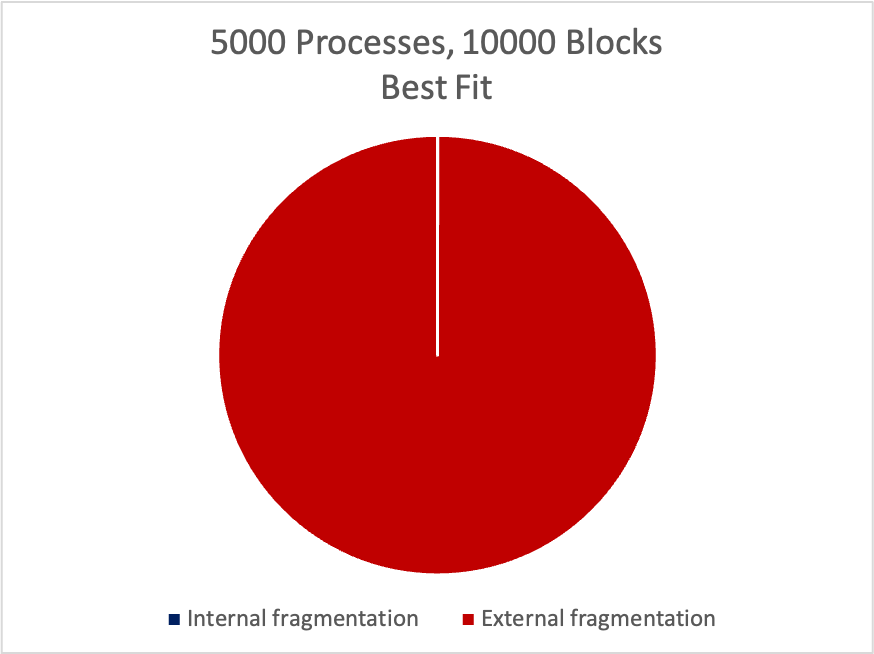
\includegraphics[width=0.95\textwidth]{10000b-5000p-best-fit.png}
    \caption{5000进程,10000内存孔Best Fit}
    \label{fig:5000p10000b-best}
\end{figure}

\begin{figure}[ht!]
    \centering
    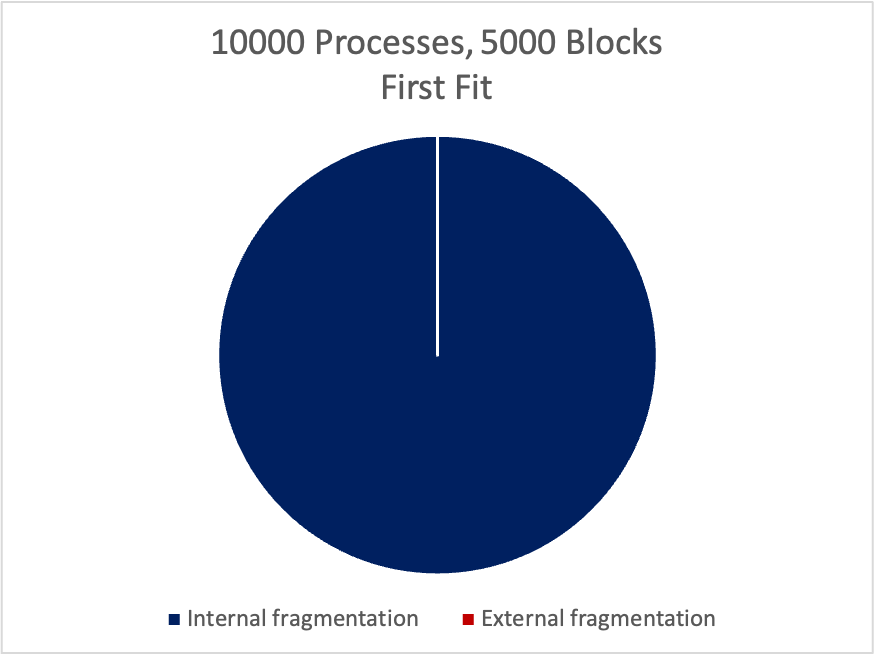
\includegraphics[width=0.95\textwidth]{5000b-10000p-first-fit.png}
    \caption{10000进程,5000内存孔First Fit}
    \label{fig:10000p5000b-first}
\end{figure}

\subsection{虚拟内存分配实验}
\subsubsection{运行环境}
程序在以下环境下构建和测试.
\begin{description}
    \item[操作系统] macOS 13.1 22C5044e arm64;
    \item[c编译器] gcc (Homebrew GCC 12.2.0) 12.2.0;
    \item[构建和测试工具] GNU Make 3.81;
    \item[文档编译工具] XeTeX 3.141592653-2.6-0.999994 (TeX Live 2022)
    \item[文本编辑器] nvim v0.8.1
    \item[调试工具] Visual Studio Code Version: 1.74.0 (Universal),
        lldb-1400.0.38.13
\end{description}

\subsubsection{程序运行方式}
程序使用make进行构建和测试. 读者优先程序和写者优先程序都会被构建在build/目录下.\par
对于程序的构建, 执行如下命令.
\begin{code}
    make
\end{code}

对于程序的执行, 可以使用如下命令:
\begin{code}
    Usage: build/main <input file> <verbose[1/0]> <replacement method[1: FIFO, 2: LRU]>
\end{code}

其中, <input file>为待访问的虚拟内存地址队列, verbose控制输出日志是详细(1)还是简略
(0); replacement method控制TLB的置换方式是FIFO还是LRU.\par

程序的测试使用本实验同时实现的数据生成器data\_gen, 根据\textbf{局部性原理}生成符
合实际情况的待访问虚拟内存地址队列, 生成的数据将保存在config/input.txt中. 可使用如下命令.

\begin{code}
    make test AMOUNT=100000 UPPER_BORDER=256 VERBOSE=0
\end{code}

执行make test的时候, 首先会使用data\_gen生成AMOUNT个待访问虚拟地址, 这些虚拟地址
连续最多有UPPER\_BORDER个在同一个帧中. VERBOSE=1可以输出更详细的日志, 即虚拟地
址, 转换到的物理地址, 以及内存中物理地址对应存储的数据.

\subsubsection{程序日志格式}
程序的日志有3种等级.\par

一级是最详细的日志, 包括虚拟地址, 物理地址和内存中物理地址对应存储的数据等信息,
当VERBOSE=1的时候输出此等级log.截取示例如下.\par
\begin{code}
    VIRTUAL MEMORY SIMULATION

    Logical pages: 256
    Page size: 256 bytes.
    Page table size: 256
    TLB size: 16 entries.
    Physical frames: 256
    Frame size: 256 bytes.
    Physical memory size: 65536 bytes.
    Virtual address[0x0003]         Physical address[0x0003]        Value[0000]
    Virtual address[0x0103]         Physical address[0x0003]        Value[0120]
    Virtual address[0x0203]         Physical address[0x0103]        Value[0070]
    Virtual address[0x0303]         Physical address[0x0203]        Value[0016]
    Virtual address[0x0403]         Physical address[0x0303]        Value[0095]
    Virtual address[0x0503]         Physical address[0x0403]        Value[0090]
    Virtual address[0x0007]         Physical address[0x0007]        Value[0017]
    Virtual address[0x0107]         Physical address[0x0007]        Value[0017]
    Virtual address[0x0207]         Physical address[0x0107]        Value[0002]
    Virtual address[0x0307]         Physical address[0x0207]        Value[0097]
    Virtual address[0x0407]         Physical address[0x0307]        Value[-122]
    Virtual address[0x0507]         Physical address[0x0407]        Value[-107]
    Virtual address[0x0003]         Physical address[0x0003]        Value[0120]
    Virtual address[0x0103]         Physical address[0x0003]        Value[0120]
    Virtual address[0x0203]         Physical address[0x0103]        Value[0070]
    Virtual address[0x0303]         Physical address[0x0203]        Value[0016]
    Virtual address[0x0403]         Physical address[0x0303]        Value[0095]
    Virtual address[0x0503]         Physical address[0x0403]        Value[0090]
    Virtual address[0x0007]         Physical address[0x0007]        Value[0017]
    Virtual address[0x0107]         Physical address[0x0007]        Value[0017]
    Virtual address[0x0207]         Physical address[0x0107]        Value[0002]
    Virtual address[0x0307]         Physical address[0x0207]        Value[0097]
    Virtual address[0x0407]         Physical address[0x0307]        Value[-122]
    Virtual address[0x0507]         Physical address[0x0407]        Value[-107]

\end{code}

二级是总结性日志, 包括本次运行使用的TLB替换算法名称, 访问的虚拟内存地址数量,
Page fault次数, Page fault比例, TLB命中次数, TLB命中率. 截取部分日志示例如下.\par

\begin{code}
    ------VIRTUAL MEMORY STATISTICS------

    Replacement method: FIFO
    Number of addresses translated: 24
    Page faults: 5
    Page fault rate: 20.833%
    TLB hits: 19
    TLB hit rate: 79.167%
    Average thme retrieving data from secondary storage: 4.600 ms

    -------------------------------------

\end{code}

第三级日志很简略, 每次程序运行会追加一行到日志文件logs/stat.log的结尾, 一行共三
个整数, 分别为访问的虚拟地址个数, Page fault次数和TLB命中次数, 示例如下.
\begin{code}
    24 5 19
\end{code}
表示进行了24次虚拟内存访问, 有5次page fault, 19次TLB命中.

\subsubsection{运行结果}
在TLB表大小为32的情况下, 分别采用FIFO和LRU的TLB替换策略, 设置不同的连续同帧虚拟
地址访问请求上界UPPER\_BORDER进行测试, 具体运行命令如下.
\begin{code}
    # 连续同帧虚拟地址上界32768
    make test UPPER_BORDER=32768

    # 连续同帧虚拟地址上界16384
    make test UPPER_BORDER=16384

    # 连续同帧虚拟地址上界4096
    make test UPPER_BORDER=4096

    # 连续同帧虚拟地址上界1024
    make test UPPER_BORDER=1024

    # 连续同帧虚拟地址上界256
    make test UPPER_BORDER=256

    # 连续同帧虚拟地址上界64
    make test UPPER_BORDER=64

    # 连续同帧虚拟地址上界16
    make test UPPER_BORDER=16

    # 连续同帧虚拟地址上界4
    make test UPPER_BORDER=4

    # 连续同帧虚拟地址上界2
    make test UPPER_BORDER=2

    # 连续同帧虚拟地址上界1
    make test UPPER_BORDER=1
\end{code}

得运行日志和Page fault, TLB hit统计如下.
\begin{itemize}
    \item 统计信息日志为logs/test\_stat.log.
    \item Page fault折线图如图~\ref{fig:page-fault统计图}.
    \item TLB命中折线图如图~\ref{fig:tlb统计图}.
\end{itemize}

\begin{figure}[ht!]
    \centering
    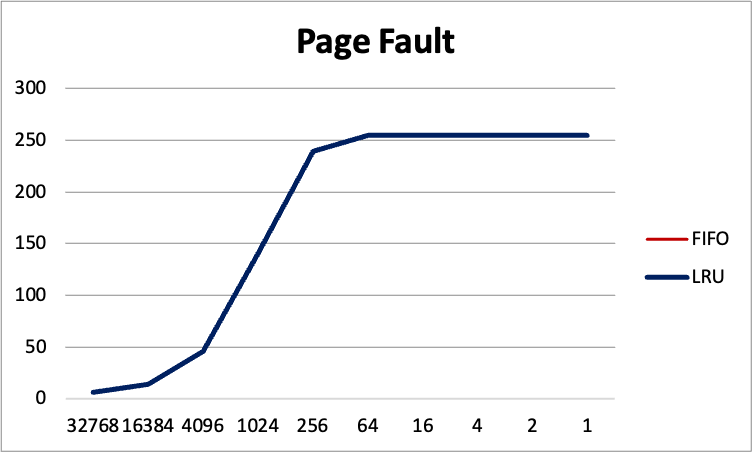
\includegraphics[width=0.95\textwidth]{page-fault.png}
    \caption{Page Fault统计图}
    \label{fig:page-fault统计图}
\end{figure}

\begin{figure}[ht!]
    \centering
    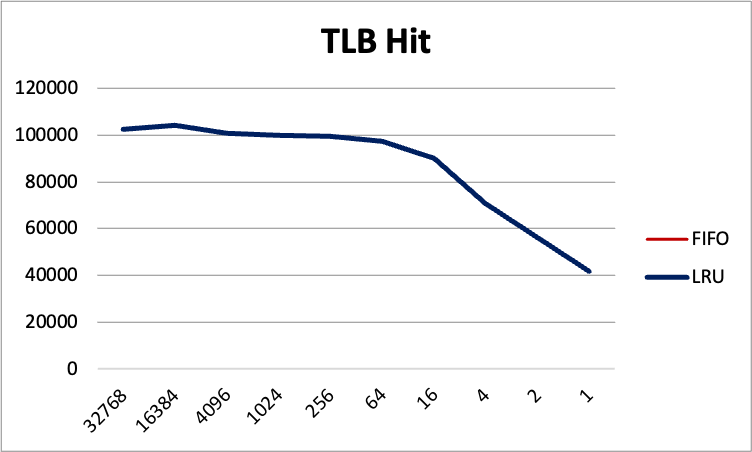
\includegraphics[width=0.95\textwidth]{tlb-hit.png}
    \caption{TLB命中统计图}
    \label{fig:tlb统计图}
\end{figure}

可以看到, 当帧内连续虚拟地址非常大的时候, 由于一帧内只有256个编址, 因此Page
fault次数很低; 随着帧内连续访问虚拟地址数量下降, Page Fault的次数迅速增加, 当将
secondary storage中全部256个帧调入DRAM后, Page fault不再增加.\par

当帧内连续虚拟地址非常大的时候, TLB命中率很高; 随着帧内连续访问虚拟地址数量下降,
TLB命中次数也逐渐下降.\par

此外, 还可以看到FIFO和LRU的TLB替换策略在Page fault和TLB命中率上表现类似, 猜测可
能是生成的数据不能很好的利用LRU的特性, 使得FIFO已经可以有足够好的表现.